%!TEX root = ../../report.tex
\section{Laser Range Sensor Model}
\label{sec:laser_range_sensor}
When A. Elfes and H. Moravec introduced the occupancy grid map they also introduced the inverse sensor model used to update a map considering the uncertainties related to measurements \cite{elfesMoravecOccGrid}. 
A sensor characteristics is described with a forward sensor model, 
\begin{equation*}
	p(z_t|m_i,x_t)
\end{equation*}
which is the probability for measuring a distance given the location of the sensor and the obstacle the measurement hits. 
The inverse sensor model,
\begin{equation*}
	p(m_i|z_t,x_t)
\end{equation*}
converts these characteristics to describe the probability for occupancy of the map given the measurement. The last term in equation \vref{eq:occupancy_update} is the log-odds version of this value.
This principle is applicable for multiple sensors but in this project it is used for LIDARs. 


\subsection{Forward Sensor Model}
LIDARs are often modeled as multiple independent beams with four different types of noise combined into one model \cite{probRob}.
The four different types is shown in figure [XXXXXX].

\begin{itemize}
	\item Gaussian measurement noise
	\item Unexpected objects
	\item Measurement failures
	\item Random measurements
\end{itemize}

\todo{Figure of noise, list to legend}

The small Gaussian measurement noise around the correct distance, arises from limited resolution of the sensor, atmospheric effects, etc. This noise is modeled as a normal distribution and should be taken into account when a sensor model is devised. 

The noise from unexpected obstacles stems from using a static map to represent a dynamic environment. When the robot senses the environment it will occasionally measure obstacles that are not present in the map, for instance moving people.

For LIDARs, failures can occur due to insufficient reflectance of light back to the sensor. 
These failures often cause a maximum range reading which are handled by removing measurements with maximum range.

The random measurements represents entirely random readings. These are modeled with a uniform distribution and should be taken into account in the sensor model.

S. Thrun proposed to learn occupancy grids from the forward sensor model with expectation-maximization \cite{probRob}.
This method reduces the effects of conflicting sensor model updates, causing incorrect addition or removal of obstacles. 
This demands for storing a batch of measurements and is computational expensive to perform. 
Therefore, it is more common to learn occupancy grids with an inverse sensor model where measurements are added incrementally according to equation \vref{eq:occupancy_update}. 

\subsection{Inverse Sensor Model}
The inverse sensor model describes the probability for a cell being occupied in an occupancy grid map given a sensor measurement and location. 
Many different inverse sensor models have been proposed to incorporate LIDAR measurements in a occupancy grid map. The individual rays are often assumed narrow and the orientation of it with respect to the robot is assumed ideal.
The simplest possible inverse sensor model is the 
ideal inverse sensor model. It assumes zero probability for occupancy before the measured distance, one at the measured distance, and $0.5$ after. The model shown in figure \vref{fig:sensor_model_std_dev01} is almost ideal.

\subsubsection{Elfes Sensor Model}
R. Merali and T. Barfoot \cite{sensorModelTuning} conducted a comparison and tuning of common inverse sensor models for laser rangefinders in a one dimensional simulated situation. It showed that the simple model with Gaussian noise proposed by A. Elfes in \cite{elfes} performed as good using only 2 parameters, as a 21 parameter approximation to the full Bayesian solution of the entire binary occupancy grid. They found that the model performed better, if the log-odds values were limited to -12.9047. This is also used in this work.

D. Joubert derives Elfes model in \cite{Joubert2014} by convolving a Gaussian function on an ideal sensor model. While this can be done analytically it is chosen to apply the yellow kernel shown in figure \vref{fig:sensor_model_std_dev01} to the ideal sensor model.
The distance to the obstacle is $0.275m$ and the standard deviation of the Gaussian kernel is $1cm$. 
SICK states the noise parameters for the S300 to be $\pm20mm$ systematic error and $\pm9mm$ statistical error, when measuring a distance of three meters \cite{lidarDatasheet}. 
Since the error might be subject variations and is used for ranges up to $30m$, the noise used in simulations for the MiR-100 is $1cm$ Gaussian noise. 
The maximum and minimal log-odds values are out of the scope, but they can be calculated from the probabilities with equation \vref{eq:occupancy_update}.


\begin{figure}[htbp]
	\centering
	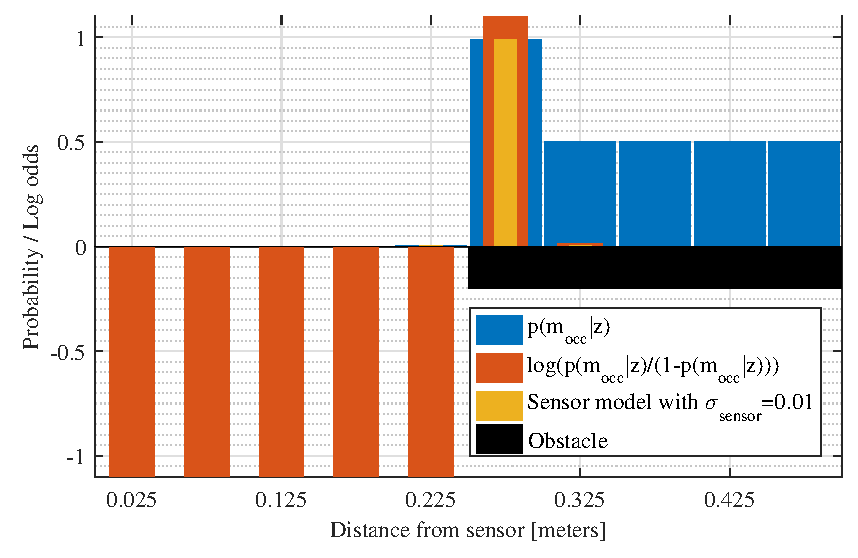
\includegraphics[scale=1.0]{figures/static_mapping/sensor_model_std_dev01}
	\caption{Elfes inverse sensor model with the used sensor's model.}
	\label{fig:sensor_model_std_dev01}
\end{figure}

Figure \vref{fig:sensor_model_std_dev025} shows an inverse sensor model with a standard deviation of $2.5cm$.
This indicates less trust in the measured distance. With this model more measurements are needed to reach as high an occupancy probability, as would be achieved with the ideal model. It can however be used to avoid overconfidence in measurements while still converging to the correct map if the measurement error is Gaussian distributed.

\begin{figure}[htbp]
	\centering
	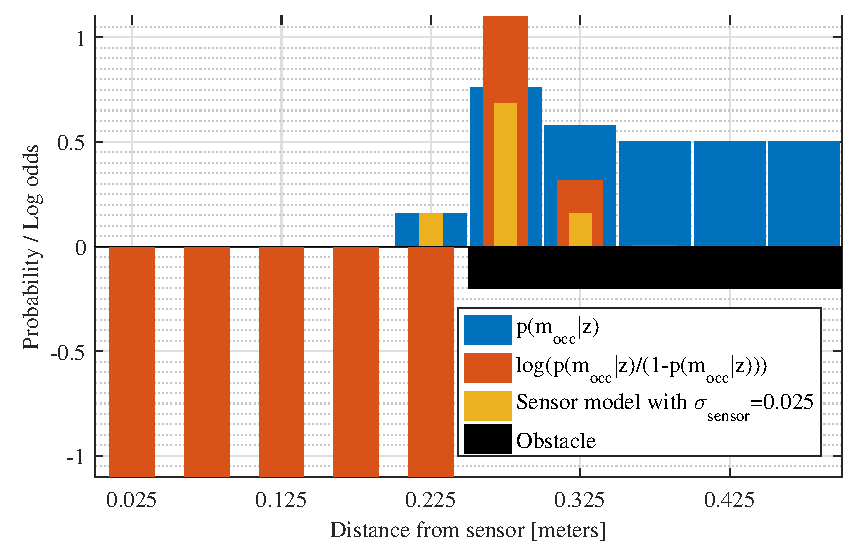
\includegraphics[scale=1.0]{figures/static_mapping/sensor_model_std_dev025}
	\caption{Elfes inverse sensor model with a larger standard deviation than that of the sensor's.}
	\label{fig:sensor_model_std_dev025}
\end{figure}

Even with the sensor noise modeled as shown in figure \ref{fig:sensor_model_std_dev01}, erroneous maps like the one shown in \ref{fig:elfes_ideal_with_poses} and \ref{fig:elfes_compare} are expected, due to localization errors.
The influence of the error could be diminished by incorporating the localization errors in the inverse sensor model.

\begin{figure}[htbp]
	\centering
	\begin{subfigure}[t]{0.45\textwidth}
		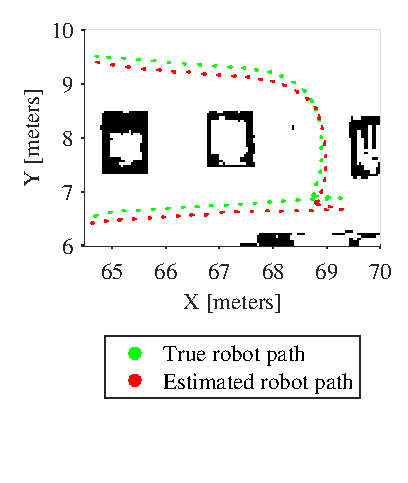
\includegraphics[scale=1.0]{figures/static_mapping/map_region_with_poses}
		\caption{Occupancy grid of the simulated world.}
		\label{fig:map_region_with_poses}
	\end{subfigure}
	\begin{subfigure}[t]{0.45\textwidth}
		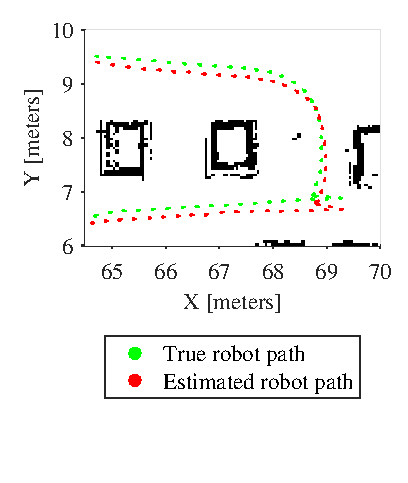
\includegraphics[scale=1.0]{figures/static_mapping/elfes_ideal_with_poses_no_decay}
		\caption{Mapped occupancy grid using the sensor model in figure \vref{fig:sensor_model_std_dev01}.}
		\label{fig:elfes_ideal_with_poses}
	\end{subfigure}
	\caption{Mapping results gained by simulating a MiR-100 robot with imprecise location.}
	\label{fig:simulated_location_error}
\end{figure}

\begin{figure}[htbp]
	\centering
	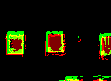
\includegraphics[width=0.5\linewidth]{figures/static_mapping/elfes_ideal_no_decay}
	\caption{Comparison between the obstacles position in figure  \vref{fig:map_region_with_poses} shown in green and the mapped obstacles in figure \vref{fig:elfes_ideal_with_poses} shown in red. The overlapping yellow regions marks areas with successful mapping.}
	\label{fig:elfes_compare}
\end{figure}

